\section{Installing KeePass}

We will cover installing KeePass on Ubuntu and Windows.

Mac OSX comes with an excellent built-in password manager called
Keychain that is just as safe. Downsides are that it isn't Open Source
and doesn't work on other systems. If you'd need to take your passwords
from one Operating System to another it is better to stick with Keepass
after all. How to use Keychain is covered in the next chapter.

\subsection{Installing KeePassX on Ubuntu}

To install on Ubuntu we will use the Ubuntu Software Center. Type
KeePass in the search field at the top right and the application
KeePassX should automatically appear in the listing.

Highlight the item (it may already be highlighted by default) and then
press `Install'. You will be asked to Authorise the installation
process:

\begin{figure}[htbp]
\centering
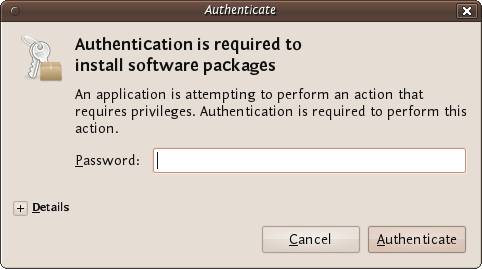
\includegraphics{keepass_1.png}
\caption{Keepass Install}
\end{figure}

Enter your password and press `Authenticate' the installation process
will then begin.

Ubuntu does not offer very good feedback to show the software is
installed. If the green progress indicator on the left has gone and the
progress bar on the right has gone then you can assumed the software is
installed.

\subsection{Installing KeePass on Windows}

First visit the \href{http://keepass.info/download.html}{KeePass
download webpage} and choose the appropriate installer. For this chapter
we are using the
\href{http://downloads.sourceforge.net/keepass/KeePass-2.15-Setup.exe}{current
installer}.

Download this to your computer then double click on the installer. You
will first be asked to select a language, we will choose English:

\begin{figure}[htbp]
\centering
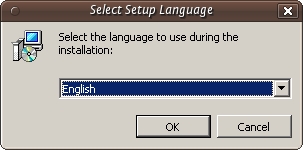
\includegraphics{keepass_2.png}
\caption{Keepass Install}
\end{figure}

Press `OK' and you will be shown the following screen:

\begin{figure}[htbp]
\centering
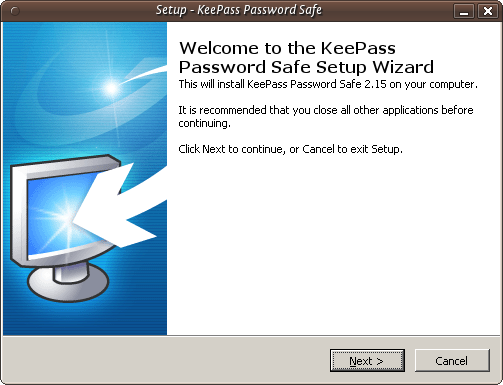
\includegraphics{keepass_3.png}
\caption{Keepass Install}
\end{figure}

Just press `Next \textgreater{}' and go to the next screen:

\begin{figure}[htbp]
\centering
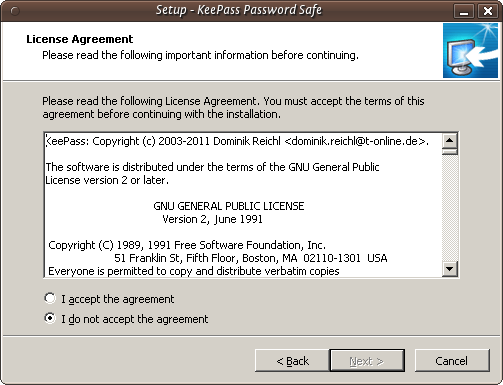
\includegraphics{keepass_4.png}
\caption{Keepass Install}
\end{figure}

In the screen shown above we must select `I accept the agreement'
otherwise we will not be able to install the software. Choose this
option and then press `Next \textgreater{}'. In the next screen you will
be asked to determine the installation location. You can leave this with
the defaults unless you have good reason to change them.

\begin{figure}[htbp]
\centering
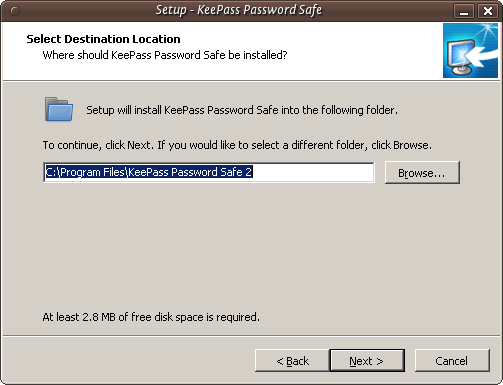
\includegraphics{keepass_5.png}
\caption{Keepass Install}
\end{figure}

Click on `Next \textgreater{}' and continue.

\begin{figure}[htbp]
\centering
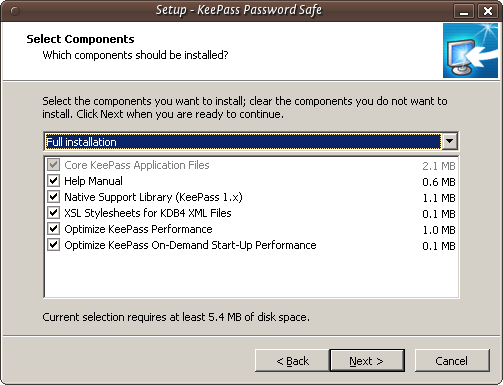
\includegraphics{keepass_6.png}
\caption{Keepass Install}
\end{figure}

The above image shows the KeePass components you can choose from. Just
leave the defaults as they are and press `Next \textgreater{}'. You will
come to a new screen:

\begin{figure}[htbp]
\centering
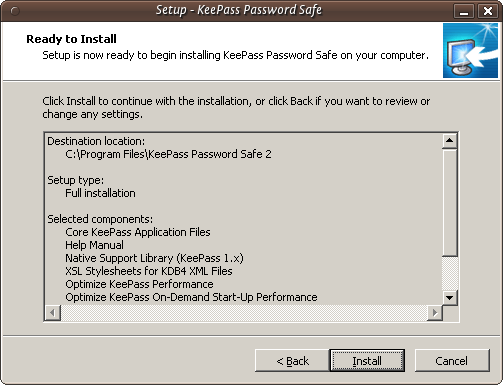
\includegraphics{keepass_7.png}
\caption{Keepass Install}
\end{figure}

This doesn't do anything but give you a summary of your options. Press
`Install' and the installation process will begin.

\begin{figure}[htbp]
\centering
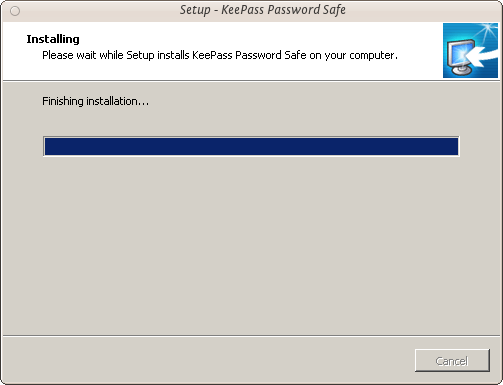
\includegraphics{keepass_8.png}
\caption{Keepass Install}
\end{figure}

\subsection{Installing KeePass on Mac OS X}

Although Keychain in Mac OS X does an excellent job of storing your
passwords, you may want to run your own password database and manager.
KeePass allows this added flexibility. First visit the KeePass download
webpage (http://keepass.info/download.html) and choose the appropriate
installer. Although the official installers are listed at the top of the
page, there are unofficial/contributed installers further down. Scroll
down to find \href{http://keepass2.openix.be/}{KeePass 2.x for Mac OS
X}:

\begin{figure}[htbp]
\centering
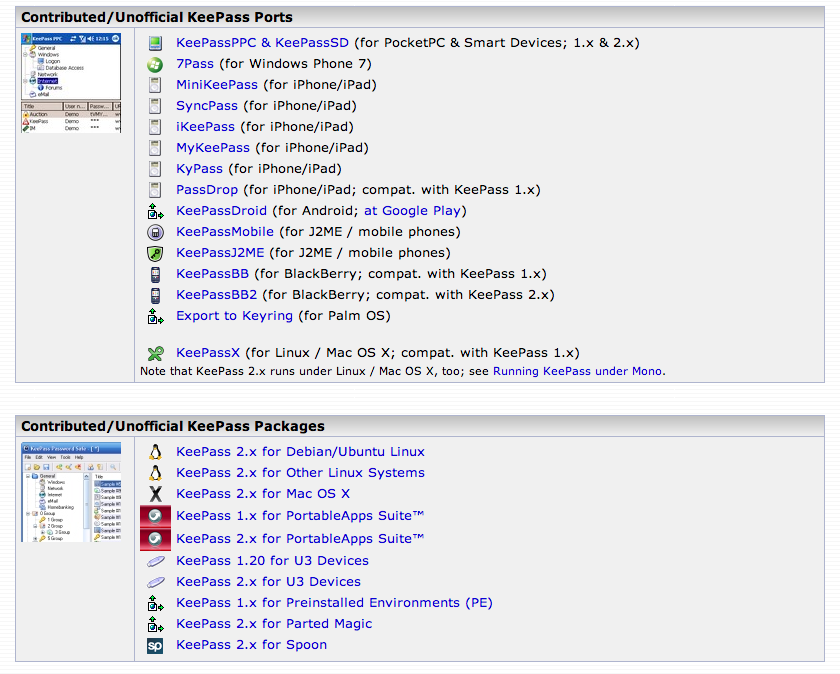
\includegraphics{keepass_9.png}
\caption{Keepass Install}
\end{figure}

As this is an external link, your browser will be redirected to
\href{http://keepass2.openix.be/}{http://keepass2.openix.be/}:

\begin{figure}[htbp]
\centering
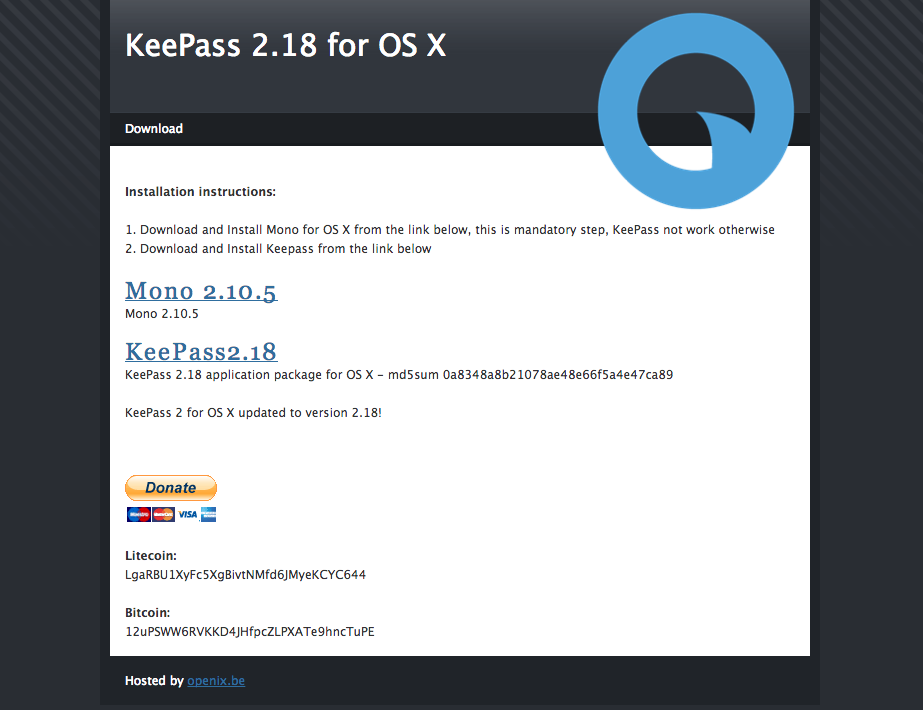
\includegraphics{keepass_10.png}
\caption{Keepass Install}
\end{figure}

Note here that you must install the Mono framework first, so that
KeePass can run in OS X. So click on each of the links
\href{http://download.mono-project.com/archive/2.10.5/macos-10-x86/0/MonoFramework-MRE-2.10.5\_0.macos10.xamarin.x86.dmg}{Mono
2.10.5} and
\href{http://keepass2.openix.be/KeePass2.18.dmg}{KeePass2.18} to
download the DMG files to your computer. Double-click on each of the
DMGs in your downloads folder to unpack the volumes to your desktop.

The Mono Package installer is called
`MonoFramework-MRE--2.10.5\_0.macos10.xamarin.x86.pkg', so double-click
on this document in the MonoFramework volume on your desktop:

\begin{figure}[htbp]
\centering
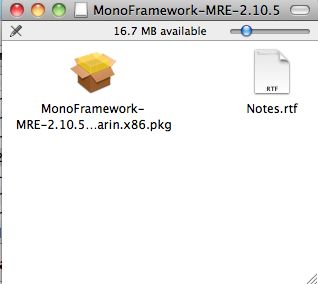
\includegraphics{keepass_11.png}
\caption{Keepass Install}
\end{figure}

The installer will open and run:

\begin{figure}[htbp]
\centering
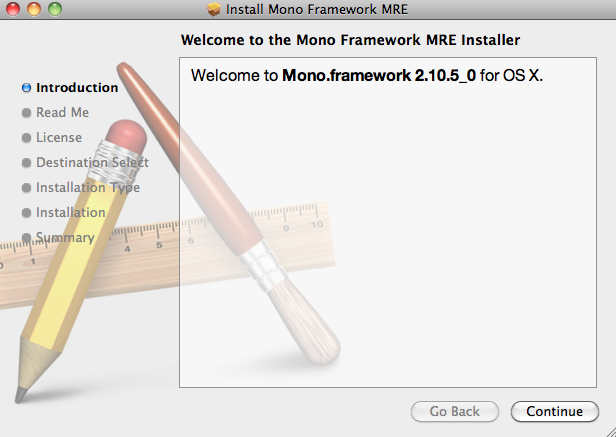
\includegraphics{keepass_12.png}
\caption{Keepass Install}
\end{figure}

Follow each of the steps by clicking `Continue', the next step being
`Read Me'. Inhere is important information such as all of the files that
the package will install, including information on how to uninstall
Mono:

\begin{figure}[htbp]
\centering
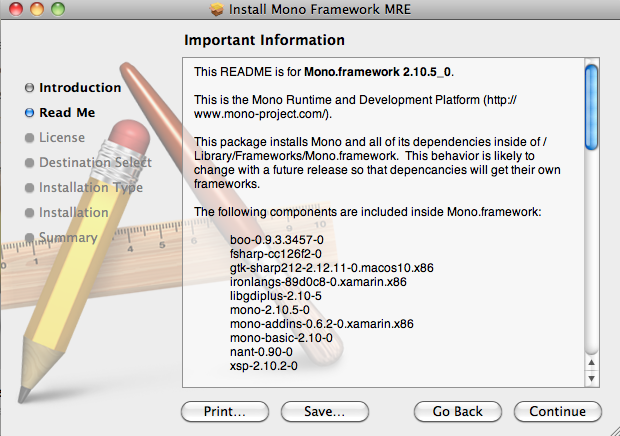
\includegraphics{keepass_13.png}
\caption{Keepass Install}
\end{figure}

Click `Continue' to the next screen, the license. Clicking `Continue' on
the license screen pops up the agree/disagree dialogue box. If you agree
with the license conditions, the installation will continue:

\begin{figure}[htbp]
\centering
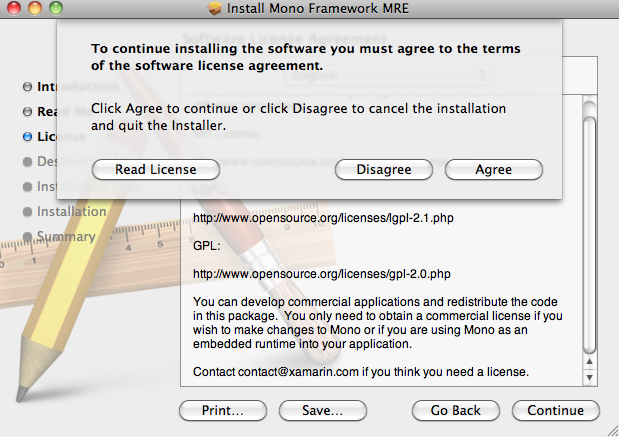
\includegraphics{keepass_14.png}
\caption{Keepass Install}
\end{figure}

The following two steps in the installation ask you to choose an
installation destination, and check there is enough space on the install
disk. When the installation has completed, you will see this screen:

\begin{figure}[htbp]
\centering
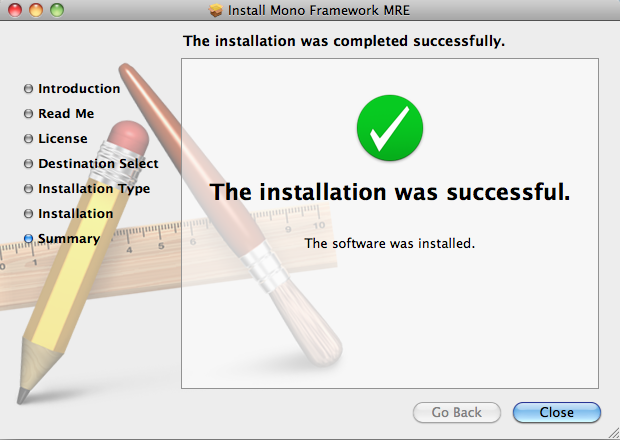
\includegraphics{keepass_15.png}
\caption{Keepass Install}
\end{figure}

Now you can quit the installer. Next take a look at the KeePass disk
image, double-click to open it, and drag the KeePass application into
your Applications folder:

\begin{figure}[htbp]
\centering
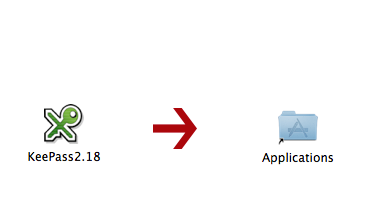
\includegraphics{keepass_16.png}
\caption{Keepass Install}
\end{figure}

Now KeePass is ready to use for Mac OS X.
